\documentclass[11pt]{article}

\usepackage[margin=2cm]{geometry}
\usepackage[T1]{fontenc}
\usepackage{graphicx}
\usepackage{amsmath}
\usepackage[super,sort&compress,comma]{natbib}
\usepackage[labelfont=bf,labelsep=period]{caption}
\usepackage[colorlinks=true,allcolors=blue]{hyperref}

\renewcommand{\figurename}{Fig.}

% Numbers the manuscript prints.
%
% Two regions. Everything between the markers below is regenerated from the
% committed result files and is never hand-edited. Anything outside them is a
% fixed convention this repository did not measure -- a value quoted from a
% cited paper -- and is hand-edited and reviewed like any other source.
%
% Each generated block declares the population its macros are measured over: the
% artifact the number came from, and the unit noun a count of that population
% takes. Two population names resolving to one artifact is a test failure.

%% POPULATION cited | artifact: npj Comput. Mater. 11, 300 (2025) | unit: rows
% Quoted from Kim & Lee's article, not measured here.
\newcommand{\npjSystems}{43}

%% POPULATION citedRelease | artifact: AI Hub dataset 71339 and Matbench v0.1 | unit: releases
% EMPD's release number, as its data description prints it, and the date on
% which the local copy was downloaded, which the archive's directory records.
% Matbench's version, as Dunn et al. name the suite that holds the task.
\newcommand{\empdRelease}{1.0}
\newcommand{\empdRetrieved}{23 December 2025}
\newcommand{\exptGapVersion}{0.1}

% ---- BEGIN GENERATED ----

%% POPULATION npjDataset | artifact: data/npj/csv/Train.csv+data/npj/csv/Val.csv | unit: rows
\newcommand{\npjDatasetRows}{71{,}633}

%% POPULATION npjTrain | artifact: data/npj/csv/Train.csv | unit: rows
\newcommand{\npjModelTrainRmse}{3.95}
\newcommand{\npjPaperTrainRmse}{3.94}

%% POPULATION npjVal | artifact: data/npj/csv/Val.csv | unit: rows
\newcommand{\npjModelRSq}{0.9946}
\newcommand{\npjModelRmse}{5.87}
\newcommand{\npjPaperRmse}{5.86}
\newcommand{\npjFeatureCount}{nine} % artifact: data/npj/csv/Val.csv | unit: features
\newcommand{\npjCompositionFeatureCount}{six} % artifact: data/npj/csv/Val.csv | unit: descriptors
\newcommand{\npjLookupRSq}{0.9924}
\newcommand{\npjMargin}{+0.0022}
\newcommand{\npjLookupRmse}{6.94}

%% POPULATION empdRes | artifact: outputs/aihub/draws.json:resistivity | unit: rows
\newcommand{\empdResBlockedHeldOutMin}{9\%}
\newcommand{\empdResBlockedHeldOutMax}{20\%}
\newcommand{\empdResRows}{58{,}937}
\newcommand{\empdResSystems}{25} % artifact: outputs/aihub/draws.json:resistivity | unit: systems
\newcommand{\empdResLookup}{0.887}
\newcommand{\empdResModel}{0.946}
\newcommand{\empdResMargin}{+0.059}
\newcommand{\empdResMarginCI}{[+0.057, +0.061]}
\newcommand{\empdResBlockedLookup}{$-$0.1}
\newcommand{\empdResBlockedLookupCI}{[$-$0.6, 0.4]}
\newcommand{\empdResBlocked}{0.1}
\newcommand{\empdResBlockedCI}{[$-$0.2, 0.4]}
\newcommand{\empdResExcess}{+0.8}
\newcommand{\empdResExcessCI}{[+0.4, +1.1]}
\newcommand{\empdResBlockedMin}{$-$0.936}
\newcommand{\empdResBlockedMax}{+0.839}
\newcommand{\empdResMarginMin}{+0.053}
\newcommand{\empdResMarginMax}{+0.064}
\newcommand{\empdResBlockedNegative}{three} % artifact: outputs/aihub/draws.json:resistivity | unit: partitions
\newcommand{\empdResBlockedPositive}{seven} % artifact: outputs/aihub/draws.json:resistivity | unit: partitions
\newcommand{\empdResValidationOnlySystems}{one} % artifact: outputs/aihub/draws.json:resistivity | unit: systems

%% POPULATION empdHard | artifact: outputs/aihub/draws.json:hardness | unit: rows
\newcommand{\empdHardBlockedHeldOutMin}{6\%}
\newcommand{\empdHardBlockedHeldOutMax}{20\%}
\newcommand{\empdHardRows}{901}
\newcommand{\empdHardSystems}{22} % artifact: outputs/aihub/draws.json:hardness | unit: systems
\newcommand{\empdHardLookup}{0.873}
\newcommand{\empdHardModel}{0.921}
\newcommand{\empdHardMargin}{+0.048}
\newcommand{\empdHardMarginCI}{[+0.035, +0.063]}
\newcommand{\empdHardMarginMin}{+0.017}
\newcommand{\empdHardBlockedLookup}{$-$4}
\newcommand{\empdHardBlockedLookupCI}{[$-$10, 0]}
\newcommand{\empdHardBlocked}{$-$6}
\newcommand{\empdHardBlockedCI}{[$-$12, $-$1]}
\newcommand{\empdHardExcess}{+7}
\newcommand{\empdHardExcessCI}{[+2, +13]}
\newcommand{\empdHardBlockedMin}{$-$23.541}
\newcommand{\empdHardBlockedMax}{+0.730}
\newcommand{\empdHardBlockedMedian}{$-$1.354}
\newcommand{\empdHardBlockedNegative}{nine} % artifact: outputs/aihub/draws.json:hardness | unit: partitions
\newcommand{\empdHardMarginMax}{+0.103}
\newcommand{\empdHardValidationOnlySystems}{four} % artifact: outputs/aihub/draws.json:hardness | unit: systems

%% POPULATION empdAmorph | artifact: outputs/aihub/draws.json:amorphous | unit: rows
\newcommand{\empdAmorphousRows}{945}

%% POPULATION npjShared | artifact: outputs/aihub/structure.json:npj_shared_measurements | unit: rows
\newcommand{\npjSharedRows}{2{,}405}
\newcommand{\npjSharedOtherRows}{157}
\newcommand{\npjSharedFactor}{0.45326}
\newcommand{\npjFactorGridLow}{0.38}
\newcommand{\npjFactorGridHigh}{0.52}
\newcommand{\npjFactorGridStep}{0.00001}
\newcommand{\npjSharedMinDecimals}{six} % artifact: outputs/aihub/structure.json:npj_shared_measurements | unit: decimals
\newcommand{\npjSharedThicknessRatio}{1.000}
\newcommand{\npjSharedThicknessRows}{2{,}289}

%% POPULATION htemRes | artifact: outputs/htem/split.json:log10_resistivity | unit: rows
\newcommand{\htemResRows}{8{,}628}
\newcommand{\htemResLibraries}{257} % artifact: outputs/htem/split.json:log10_resistivity | unit: libraries
\newcommand{\htemResRandomLookup}{0.84}
\newcommand{\htemResRandomModel}{0.90}
\newcommand{\htemResBlockedLookup}{0.14}
\newcommand{\htemResBlockedLookupCI}{[$-$0.06, 0.31]}
\newcommand{\htemResBlockedModel}{0.36}
\newcommand{\htemResBlockedModelCI}{[0.20, 0.48]}
\newcommand{\htemResMargin}{+0.057}
\newcommand{\htemResMarginCI}{[+0.042, +0.075]}
\newcommand{\htemResExcess}{+0.48}
\newcommand{\htemResExcessCI}{[+0.37, +0.62]}
\newcommand{\htemResBeyondHalf}{+0.28}
\newcommand{\htemResBeyondHalfCI}{[+0.11, +0.48]}
\newcommand{\htemResFallExcess}{+0.16}
\newcommand{\htemResFallExcessCI}{[+0.04, +0.29]}
\newcommand{\htemResFillFallLo}{+0.037}
\newcommand{\htemResMarginMin}{+0.051}
\newcommand{\htemResMarginMax}{+0.064}

%% POPULATION htemGap | artifact: outputs/htem/split.json:direct_band_gap | unit: rows
\newcommand{\htemGapRows}{5{,}264}
\newcommand{\htemGapLibraries}{156} % artifact: outputs/htem/split.json:direct_band_gap | unit: libraries
\newcommand{\htemGapRandomLookup}{0.66}
\newcommand{\htemGapRandomLookupCI}{[0.56, 0.74]}
\newcommand{\htemGapRandomLookupLo}{0.559}
\newcommand{\htemGapRandomModel}{0.78}
\newcommand{\htemGapBlockedLookup}{0.2}
\newcommand{\htemGapBlockedLookupCI}{[$-$0.1, 0.4]}
\newcommand{\htemGapBlockedModel}{0.47}
\newcommand{\htemGapBlockedModelCI}{[0.33, 0.58]}
\newcommand{\htemGapMargin}{+0.12}
\newcommand{\htemGapMarginCI}{[+0.09, +0.16]}
\newcommand{\htemGapExcess}{+0.19}
\newcommand{\htemGapExcessCI}{[+0.10, +0.29]}
\newcommand{\htemGapBeyondHalf}{+0.16}
\newcommand{\htemGapBeyondHalfCI}{[$-$0.01, +0.37]}
\newcommand{\htemGapFallExcess}{+0.19}
\newcommand{\htemGapFallExcessCI}{[+0.06, +0.33]}
\newcommand{\htemGapFillFallLo}{+0.018}
\newcommand{\htemGapMarginMin}{+0.114}
\newcommand{\htemGapMarginMax}{+0.130}
\newcommand{\htemGapFirstMargin}{+0.13}
\newcommand{\htemGapFirstMarginCI}{[+0.09, +0.17]}

%% POPULATION htemResAblation | artifact: outputs/htem/ablation.json:log10_resistivity | unit: rows
\newcommand{\htemResRandomTuned}{0.90}
\newcommand{\htemResBlockedTuned}{0.39}
\newcommand{\htemResExcessTuned}{+0.45}
\newcommand{\htemResExcessTunedCI}{[+0.35, +0.56]}
\newcommand{\htemResRandomBoosted}{0.90}
\newcommand{\htemResBlockedBoosted}{0.33}
\newcommand{\htemResExcessBoosted}{+0.51}
\newcommand{\htemResExcessBoostedCI}{[+0.39, +0.64]}

%% POPULATION htemGapAblation | artifact: outputs/htem/ablation.json:direct_band_gap | unit: rows
\newcommand{\htemGapRandomTuned}{0.79}
\newcommand{\htemGapBlockedTuned}{0.55}
\newcommand{\htemGapExcessTuned}{+0.11}
\newcommand{\htemGapExcessTunedCI}{[+0.03, +0.20]}
\newcommand{\htemGapRandomBoosted}{0.79}
\newcommand{\htemGapBlockedBoosted}{0.48}
\newcommand{\htemGapExcessBoosted}{+0.18}
\newcommand{\htemGapExcessBoostedCI}{[+0.09, +0.27]}

%% POPULATION exptGap | artifact: outputs/expt_gap/control.json | unit: rows
\newcommand{\exptGapRows}{4{,}604}
\newcommand{\exptGapLookup}{0.26}
\newcommand{\exptGapLookupCI}{[0.19, 0.32]}
\newcommand{\exptGapModel}{0.48}
\newcommand{\exptGapMargin}{+0.23}
\newcommand{\exptGapMarginCI}{[+0.17, +0.29]}
\newcommand{\exptGapMarginMin}{+0.193}
\newcommand{\exptGapMarginMax}{+0.267}
\newcommand{\exptGapFirstMargin}{+0.19}
\newcommand{\exptGapFirstMarginCI}{[+0.13, +0.26]}
\newcommand{\exptGapZeroShare}{53\%}
\newcommand{\exptGapNonzeroRows}{2{,}154} % artifact: outputs/expt_gap/control.json | unit: compounds
\newcommand{\exptGapNonzeroLookup}{0.51}
\newcommand{\exptGapNonzeroLookupCI}{[0.45, 0.56]}
\newcommand{\exptGapNonzeroLookupHi}{0.562}
\newcommand{\exptGapNonzeroMargin}{+0.20}
\newcommand{\exptGapNonzeroMarginCI}{[+0.14, +0.26]}

%% POPULATION programs | artifact: reproduce/make_parameters.py | unit: sources
\newcommand{\programCount}{two}

%% POPULATION design | artifact: reproduce/ | unit: settings
\newcommand{\mlpFirstLayer}{128} % artifact: reproduce/ | unit: units
\newcommand{\mlpSecondLayer}{64} % artifact: reproduce/ | unit: units
\newcommand{\mlpDropout}{0.3}
\newcommand{\mlpEpochs}{200} % artifact: reproduce/ | unit: epochs
\newcommand{\mlpPatience}{30} % artifact: reproduce/ | unit: epochs
\newcommand{\mlpBatchSize}{32} % artifact: reproduce/ | unit: rows
\newcommand{\mlpLearningRate}{$10^{-3}$}
\newcommand{\mlpWeightDecay}{$10^{-5}$}
\newcommand{\mlpLrFactor}{0.5}
\newcommand{\mlpLrPatience}{10} % artifact: reproduce/ | unit: epochs
\newcommand{\mlpMaxGradNorm}{1.0}
\newcommand{\randomPairs}{five} % artifact: outputs/ (the pairs that the result files score) | unit: pairs
\newcommand{\libraryDatasets}{three} % artifact: outputs/ (the pairs that the result files score) | unit: datasets
\newcommand{\largestRandomMargin}{+0.12} % artifact: outputs/ (the pairs that the result files score) | unit: settings
\newcommand{\largestRandomMarginPair}{HTEM-DB band gap} % artifact: outputs/ (the pairs that the result files score) | unit: settings
\newcommand{\blockedPairs}{four} % artifact: outputs/ (the pairs that the result files score) | unit: pairs
\newcommand{\blockedDatasets}{two} % artifact: outputs/ (the pairs that the result files score) | unit: datasets
\newcommand{\splitDraws}{ten} % artifact: reproduce/ | unit: partitions
\newcommand{\splitInits}{three} % artifact: reproduce/ | unit: times
\newcommand{\heldOutShare}{15\%}
\newcommand{\empdTrainShare}{70\%}
\newcommand{\empdStopShare}{15\%}
\newcommand{\npjCommit}{8c2f808}
\newcommand{\htemFolds}{five} % artifact: reproduce/ | unit: folds
\newcommand{\htemTrees}{200} % artifact: reproduce/ | unit: trees
\newcommand{\htemNoTemperature}{$-$1}
\newcommand{\htemNoTemperatureAlternatives}{0, $-$100 or $-$1000}
\newcommand{\htemNoTemperatureShift}{0.0049} % artifact: outputs/htem/split.json | unit: settings
\newcommand{\htemNoTemperatureLookupShift}{0.069} % artifact: outputs/htem/split.json | unit: settings
\newcommand{\empdElementCount}{15} % artifact: reproduce/ | unit: elements
\newcommand{\empdDescriptorCount}{six} % artifact: reproduce/ | unit: descriptors
\newcommand{\htemTunedTrees}{400} % artifact: reproduce/ | unit: trees
\newcommand{\htemSearchBudget}{25} % artifact: reproduce/ | unit: configurations
\newcommand{\htemInnerFolds}{four} % artifact: reproduce/ | unit: folds
\newcommand{\htemBoostRounds}{1{,}000} % artifact: reproduce/ | unit: rounds
\newcommand{\htemForestFeatureShares}{0.05, 0.15, 0.3, 0.5 or 1.0}
\newcommand{\htemForestMinLeaf}{1, 3, 10, 30 or 100}
\newcommand{\htemBoostRates}{0.01, 0.03, 0.06, 0.12 or 0.25}
\newcommand{\htemBoostLeaves}{3, 7, 15, 63 or 255}
\newcommand{\htemBoostPenalty}{1.0}
\newcommand{\bootstrapReplicates}{2{,}000} % artifact: reproduce/ | unit: resamples
\newcommand{\bootstrapLevel}{95}

%% POPULATION software | artifact: requirements.txt | unit: versions
\newcommand{\numpyVersion}{1.26.4}
\newcommand{\scipyVersion}{1.13.1}
\newcommand{\sklearnVersion}{1.6.1}
\newcommand{\torchVersion}{2.8.0}

% ---- END GENERATED ----


\title{Two reporting checks for machine learning accuracy on combinatorial
materials libraries}
\author{Sungwoo Kang$^{1,\ast}$ and Jong-Kook Kim$^{2,\ast}$}
\date{}

\begin{document}
\maketitle

\noindent$^{1}$Department of Electrical and Computer Engineering, Korea
University, Seoul, Republic of Korea.\\
$^{2}$School of Electrical Engineering, Korea University, Seoul, Republic of
Korea.\\
$^{\ast}$Corresponding authors. E-mail: krml919@korea.ac.kr (S.K.);
jongkook@korea.ac.kr (J.-K.K.)

\begin{abstract}
\noindent On combinatorial libraries (composition-graded thin films measured at
many positions), a random partition tests a model on positions adjacent to
training positions, so the model's $R^2$ can overstate accuracy on new
libraries. A nearest-neighbor lookup reaches most of the model's $R^2$ on
\libraryDatasets\ datasets. On the one dataset that records each position's
library, excluding libraries from training lowers the model's $R^2$ by more than
the model gains over the lookup.
\end{abstract}

\label{par:intro}
Machine-learning models that predict a material's properties from its
composition are used to choose which materials to synthesize and measure
next.\cite{meredig2018extrapolation,thelen2025electrocatalyst} Such a model is
used on unmeasured materials, which can differ from every material in its
training data. However, a model's score on test data drawn at
random from its dataset can overestimate its accuracy on such
materials.\cite{meredig2018extrapolation}

High-throughput experiments supply large datasets for training machine-learning
models of material properties.\cite{green2013combinatorial,zakutayev2018htem}
Combinatorial synthesis, one such experiment, co-deposits several elements
onto one substrate to make a library, a film whose composition varies
continuously across the substrate.\cite{green2013combinatorial}
Combinatorial datasets are assembled from many libraries as tables in which
each row describes the composition and the measured properties at one position
on a library.

A model trained on a combinatorial dataset predicts one measured property, its
target, from features of each row such as its composition. Rows from
the same library are autocorrelated, which means that rows at adjacent
positions have similar compositions and targets. A random partition of
the rows puts some positions of each library in the test set and keeps other
positions in training, so the training row nearest to a test row in
composition can be an adjacent position on the same library. The test score
under a random partition can therefore overestimate the model's accuracy on a
library excluded from training, such as a library of new materials chosen with
the model. Fields whose data are autocorrelated use a blocked
partition instead, which keeps each group of related rows entirely in training
or in the test
set.\cite{roberts2017crossvalidation,wu2018moleculenet,meredig2018extrapolation}
In a combinatorial dataset, the related rows are those of one library.

We found three reports that test models on combinatorial datasets under a
blocked partition and score the groups excluded from training by the root mean
squared error (RMSE) or the mean absolute
error.\cite{zakutayev2018htem,thelen2025electrocatalyst,kim2025descriptors}
None of the three reports gives the coefficient of determination $R^2$
under its blocked partition, so none shows how much of a random-partition $R^2$
a model keeps on a library excluded from training.

We therefore propose two checks of a model's random-partition $R^2$. The first
check
scores a lookup on the model's test rows. The lookup, the
nearest-neighbor baseline of Meredig et al.,\cite{meredig2018extrapolation}
copies the target of the training row nearest to each test row in the model's
features. The
lookup fits no parameters to the target, so its $R^2$ comes only from training
rows that resemble the test rows, such as adjacent positions on the same
library. The model's margin relative to the lookup, the model's $R^2$
minus the lookup's, measures what the model adds to copying such rows. The
second check reports the drop in the model's $R^2$ from the random partition
to a blocked partition and compares it with the margin. Under the first check, the lookup reaches most of
the model's random-partition $R^2$ on \libraryDatasets\ combinatorial datasets. On the one dataset that records each row's library, excluding libraries
from training lowers the model's $R^2$ by more than the model gains over the
lookup.

\label{par:margin}
The first check scores the lookup and a model on the High Throughput
Experimental Materials Database (HTEM-DB),\cite{zakutayev2018htem} the
Experimental Materials Property Database (EMPD)\cite{aihubMaterials} and the
dataset that Kim and Lee released,\cite{kim2025descriptors}
\libraryDatasets\ combinatorial datasets. Each check is computed per pair of a
dataset and a measured property. The pairs are resistivity on each dataset,
hardness on EMPD and band gap on HTEM-DB, \randomPairs\ pairs in all. The model
is Kim and Lee's published network on their dataset, a neural network that we
train on EMPD and an untuned random forest that we train on HTEM-DB. Under a
random partition, the lookup reaches most of the model's $R^2$ on all
\randomPairs\ pairs (Table~\ref{tab:main}a, Fig.~\ref{fig:split}). The
margin ranges from \npjMargin\ on Kim and Lee's
dataset to \largestRandomMargin\ on \largestRandomMarginPair. On EMPD hardness,
a single partition's margin can be more than twice the mean over the partitions
(Supplementary Information Section~S1). The margin on Kim
and Lee's dataset separates the lookup's $R^2$ of \npjLookupRSq\ from their
network's \npjModelRSq\ on their validation set, which is their test set. On
those rows, RMSE separates the two more clearly (Supplementary Information
Section~S3).

The measured band gaps of Matbench\cite{zhuo2018bandgap,dunn2020matbench} are a
control dataset without libraries, on which we test whether the lookup's $R^2$
comes from the libraries and whether the model's margin is wider without them.
On Matbench, the lookup's mean $R^2$ is lower and the mean margin wider than on
any of the \randomPairs\ pairs in Table~\ref{tab:main}a. Matbench matches HTEM-DB band gap
in the kind of property, model and partition, but the band gap of
\exptGapZeroShare\ of its compounds is zero, which can lower the lookup's score and so widen
the margin. On Matbench, the wider margin is not established (Supplementary
Information Section~S1).

\label{par:partition}
The second check runs on HTEM-DB and EMPD, the \blockedDatasets\ datasets whose
releases record each row's library or its alloy system, the set of elements from
which a library was deposited. On HTEM-DB, which records each row's library, the
model's $R^2$ falls from \htemResRandomModel\ to
\htemResBlockedModel\ on resistivity and from \htemGapRandomModel\ to
\htemGapBlockedModel\ on band gap when whole libraries are excluded from
training (Fig.~\ref{fig:split}). The lookup's $R^2$ on HTEM-DB falls further than the model's on both properties, by
\htemResFallExcess\ \htemResFallExcessCI\ (bracketed ranges are \bootstrapLevel\%
percentile bootstrap intervals) on resistivity and \htemGapFallExcess\
\htemGapFallExcessCI\ on band gap, so the lookup depends more than the model on
training rows from the test row's own library. The lookup's
blocked-partition $R^2$ on resistivity also lies below half of its
random-partition $R^2$, by \htemResBeyondHalf\ \htemResBeyondHalfCI, so on
resistivity most of the lookup's random-partition $R^2$ depends on training
rows from the test row's own library. On band gap, the lookup's blocked-partition $R^2$ lies below half of its
random-partition $R^2$ by \htemGapBeyondHalf\ \htemGapBeyondHalfCI, an interval
that includes zero, so on band gap that conclusion is not established.

The excess, a pair's drop minus its margin, is positive on all
\blockedPairs\ pairs of HTEM-DB and EMPD
(Table~\ref{tab:main}b). Both HTEM-DB intervals for the excess exclude zero. EMPD's tables record no library, so its blocked partitions exclude whole alloy
systems from training. The model's blocked $R^2$ on EMPD varies so widely across
these partitions that its mean describes no typical partition (Supplementary
Information Section~S1). On EMPD, the excess is also positive for both properties under each of
\splitDraws\ blocked partitions. However, the EMPD intervals resample only those partitions and so omit how
the excess would vary over other alloy systems, whereas the HTEM-DB intervals
resample libraries. The positive excess is therefore established on HTEM-DB
alone.

Three limits bound what the margins and the drops show. First, a drop comes both from
the adjacent training positions that a blocked partition removes and from the
difficulty of predicting an excluded library's property from composition and a
few processing variables alone.
Neither the drop nor the excess therefore measures the contribution of
adjacent positions alone. Second, the positive excess on HTEM-DB is shown only for
the untuned random forest that we train on HTEM-DB and for two tuned models, a
forest and a gradient-boosting machine (Supplementary Information Section~S2), so other models could give a smaller excess. Third, the
\randomPairs\ pairs come from only
\programCount\ sources of libraries, because EMPD and Kim and Lee's dataset
share measurements (see Methods section), so the pairs are not \randomPairs\
independent tests.

\label{par:conclusion}
Both checks can be reported alongside a random-partition $R^2$ on other
combinatorial datasets, because the first needs no training and the second
needs only a model's predictions on groups excluded from its training,
predictions that each of the three reports already scores by RMSE or mean
absolute error.

\section*{Methods}
\label{sec:methods}

\subsection*{Datasets}
\label{sec:datasets}

Kim and Lee's dataset records the resistivity of thin-film alloys at
\npjDatasetRows\ positions on libraries, one row per
position.\cite{kim2025descriptors} Kim and Lee release the dataset as
two files, a training file and a validation file that serves as their test
set. Their article groups the rows into
alloy systems, which neither file records. Kim and Lee's public repository, which we use at its commit \npjCommit,
contains the two files, their network's weights and the code that computes the
network's predictions.

EMPD records resistivity at \empdResRows\ positions on libraries of
\empdResSystems\ alloy systems and hardness at \empdHardRows\ positions of
\empdHardSystems\ systems, one row per position.\cite{aihubMaterials} We use
its release \empdRelease, which we downloaded on \empdRetrieved\ from AI Hub, a
Korean government data platform. The release's three tables record resistivity, hardness, and an
amorphous or crystalline label. The label, recorded for \empdAmorphousRows\ rows, is a classification target that $R^2$
cannot score, so we score no model on it. The release splits each table in row order into a training part
and a validation part, which together contain the rows counted above, and
withholds a third part for testing.


The release also includes the raw measurements from which its tables derive.
Unlike the tables, these
raw measurements are filed by library. Each library has a file of
its measured resistances, which no row of the tables names.

EMPD and Kim and Lee's dataset share measurements. EMPD's construction
guideline, which describes how the release's data were produced, states that
the Applied Mechanics and Materials Design Laboratory of Dongwoo Lee at
Sungkyunkwan University deposited and measured
EMPD's films.\cite{aihubGuideline} Dongwoo Lee is the second of the two
authors of Kim and Lee's article. We therefore compared the two datasets'
resistivity values through the measured resistance, which EMPD multiplies by the film's
thickness and by a conversion factor to give each resistivity value. Kim and
Lee's files record resistivity and thickness, so dividing their resistivity by
their thickness and by that factor should recover the resistance. We compared
the quotient with the raw EMPD resistances that are recorded with \npjSharedMinDecimals\ or more
decimals and that occur at only one position in the release, because a shorter
value can match by chance and a repeated value identifies no single position. Kim
and Lee's resistivity, divided by their thickness and by \npjSharedFactor,
reproduces such a resistance to its last recorded decimal on \npjSharedRows\ of
their rows, and no other divisor near it reproduces as many (Supplementary
Information Section~S3). The \npjSharedRows\ rows therefore lie on
libraries that both datasets contain, so we count the two datasets as one source of libraries, because two datasets
that share libraries are not independent sources.

HTEM-DB records resistivity and, at some of the same positions, an optical
direct band gap.\cite{zakutayev2018htem} Through its public interface we
retrieved \htemResRows\ rows over \htemResLibraries\ libraries that record
composition and resistivity, one row per position. Of those rows, \htemGapRows\ over
\htemGapLibraries\ libraries record a band gap. We model HTEM-DB resistivity as
its base-10 logarithm, because its values span many powers of ten.

The control dataset is not a set of libraries. It is the experimental band-gap
task of the Matbench benchmark suite, version
\exptGapVersion,\cite{zhuo2018bandgap,dunn2020matbench} whose \exptGapRows\
rows are compounds with a measured band gap, as on HTEM-DB's band-gap rows.

\subsection*{Features}
\label{sec:features}

Each dataset's features are the composition of each row, descriptors computed
from the composition, or both. The features of the three combinatorial datasets
also include processing variables such as film thickness.
Of Kim and Lee's \npjFeatureCount\ features,
\npjCompositionFeatureCount\ are descriptors computed from composition alone. The
other features are the processing variables film thickness, deposition rate
and homologous temperature. The homologous temperature is the deposition temperature divided by the
composition-weighted mean of the elements' melting temperatures. On EMPD, the features are the atomic percent of each of \empdElementCount\ elements, the
film thickness and the \empdDescriptorCount\ descriptors that EMPD's tables
contain. EMPD's descriptors are the mean atomic radius, the atomic size mismatch, the mixing
enthalpy, the mean electronegativity, the electronegativity difference and the
number of elements. EMPD's construction guideline states that the composition and the thickness at
each measured position are interpolated linearly from the library's own
composition and thickness measurements,\cite{aihubGuideline} so a row's
composition and thickness vary smoothly between adjacent positions of a
library. A test row's nearest training row in the features that we use on EMPD
can therefore be
an adjacent position of its own library, whose target the lookup copies.

On HTEM-DB, the features are the atomic fraction of each element measured by
X-ray fluorescence, the film thickness and the deposition temperature. A row
that records no deposition temperature takes \htemNoTemperature\ instead, a
value below every recorded temperature (Supplementary Information Section~S3
replaces it by other such values). On Matbench, the features are the atomic
fraction of each element in the compound's formula.

\subsection*{Lookup and models}
\label{sec:predictors}

The lookup is the nearest-neighbor baseline of Meredig et
al.,\cite{meredig2018extrapolation} which we run with
SciPy~\scipyVersion.\cite{virtanen2020scipy} The lookup first rescales each
feature to span 0 to 1 over the training rows, except that a feature constant
over the training rows only has that constant subtracted. The lookup then predicts each
test row by copying the target of the training row at the smallest $L_1$
distance in the rescaled features. The lookup fits no parameters to the
target, because the rescaling uses no target value. If several training
rows share the smallest distance, as when two training rows record identical
features, the lookup predicts the mean of their targets.

On Kim and Lee's dataset, the model is their published network, a multilayer
perceptron\cite{rumelhart1986backprop}, which we evaluate from their released weights with
NumPy~\numpyVersion.\cite{harris2020numpy} As their published code does, we
rescale the network's features to span 0 to 1 over the training and validation
rows together.\cite{kim2025descriptors} This rescaling therefore leaks
information into the network's inputs from the validation rows, on which the
network is scored, whereas the lookup's rescaling uses the training rows alone,
so this leakage can raise the network's score and not the lookup's. The margin on Kim and
Lee's dataset can therefore overstate what the network adds to copying the
nearest training row. We nevertheless keep this rescaling, because a margin
narrower than the one in Table~\ref{tab:main}a would only strengthen the
finding that the lookup reaches most of the network's $R^2$, and because with this rescaling our evaluation reproduces
the RMSE that the article reports on each of the two files to within one unit
of its last reported digit. The network's RMSE
is \npjModelTrainRmse~$\mu\Omega\cdot$cm on the training file and
\npjModelRmse~$\mu\Omega\cdot$cm on the validation file, compared with the
article's \npjPaperTrainRmse\ and \npjPaperRmse.

On EMPD, HTEM-DB and Matbench, we train our own model. On EMPD, the model is a neural network, a
multilayer perceptron with hidden layers of \mlpFirstLayer\ and \mlpSecondLayer\ units and a dropout
rate of \mlpDropout. We train one perceptron for each property with
PyTorch~\torchVersion.\cite{paszke2019pytorch} Each hidden layer is followed by
batch normalization. Each perceptron trains with the AdamW optimizer, at a
learning rate of \mlpLearningRate\ and a weight decay of \mlpWeightDecay, on
batches of \mlpBatchSize\ rows, with the gradient norm clipped at
\mlpMaxGradNorm, for at most \mlpEpochs\ epochs. Its training loss is the mean squared error on its target after an affine
rescaling over the training rows, a rescaling that changes no test $R^2$. The early-stopping rows are a separate set
of rows that the partition keeps apart from the training and test rows and that
the lookup does not use. The perceptron's loss on the early-stopping rows is the mean of the mean
squared errors of its batches. Training stops after \mlpPatience\ epochs
without a new lowest value of that loss. The perceptron keeps the weights of
the epoch at which that loss was lowest. The
learning rate is multiplied by \mlpLrFactor\ whenever that loss has not reached
a new lowest value for more than \mlpLrPatience\ epochs. A partition of EMPD splits
the rows of all three of its tables at once. Each perceptron rescales its
features by their median and interquartile range over every training row of its partition, whichever table the row comes from. A feature whose interquartile
range is zero only has its median subtracted.
We train each perceptron \splitInits\ times on each random and each blocked partition, each time from
different random starting weights. A partition's score is the mean of the
resulting $R^2$ values. On
HTEM-DB and Matbench, the model is an untuned random
forest\cite{breiman2001randomforests} of \htemTrees\ decision trees from
scikit-learn~\sklearnVersion,\cite{pedregosa2011sklearn} with every other
hyperparameter at its default value. We also replace the untuned forest on HTEM-DB with two
models tuned inside their training folds, a random forest and a gradient-boosting
machine,\cite{friedman2001gradient} both from scikit-learn, to find whether the
positive excess on HTEM-DB depends on the untuned forest (Supplementary
Information Section~S2).

\subsection*{Partitions and comparisons}
\label{sec:protocol}

On Kim and Lee's dataset we use the random partition that their training and
validation files define. HTEM-DB publishes no partition, so we draw its random
partitions ourselves. EMPD's split in row order is not a random partition of
the rows (Supplementary Information Section~S3), so we pool the training and
validation parts that the release publishes and draw EMPD's random partitions
ourselves too. We draw \splitDraws\ random partitions of EMPD, of
HTEM-DB and of Matbench, each from its own seed. On EMPD, a random partition assigns \empdTrainShare\ of each property's rows
to training, \empdStopShare\ to the early-stopping rows and \heldOutShare\ to
the test set. On HTEM-DB and Matbench, each seed splits the rows into
\htemFolds\ cross-validation folds instead, so every row is predicted exactly
once under each partition, by the forest trained without the row's fold. Because
every row then has one prediction under each partition, the intervals on these
two datasets can resample the predictions by library or by compound. A
score on EMPD, HTEM-DB or Matbench is the mean over that dataset's partitions.

On HTEM-DB, the blocked partition assigns whole libraries to \htemFolds\
folds, as many folds as its random partitions have, so that the two differ only
in their grouping. The blocked partition needs no seed, because it assigns the libraries
in descending order of size, each to the fold that contains the fewest rows so
far. On EMPD, each library belongs to one alloy
system, so a blocked partition of whole alloy systems also excludes whole
libraries from training. From the seed of each random partition, we draw one
blocked partition of EMPD, whose training, early-stopping and test parts have
the same intended shares of each property's rows as those of a random partition, so that
the two differ mainly in their grouping. The blocked partition takes EMPD's
alloy systems one at a time, in an order that the seed shuffles. Each system
goes to the part whose share of some property's rows falls furthest below the
part's intended share.
Because the alloy systems enter the test set whole, the
test set contains between \empdResBlockedHeldOutMin\ and
\empdResBlockedHeldOutMax\ of the resistivity rows and between
\empdHardBlockedHeldOutMin\ and \empdHardBlockedHeldOutMax\ of the hardness rows,
depending on the partition, so a blocked partition of EMPD also differs from a
random one in the size of its test set.

Under every blocked partition of HTEM-DB and EMPD, we score the lookup and the
model, which keeps the hyperparameters that it has under the random
partitions. We do not apply the blocked partition to Matbench,
which contains no libraries. Nor do we apply it to Kim and Lee's
dataset, whose files record no group and whose model is their published
network rather than one we train.

A partition's $R^2$ is computed over all of its test rows, relative to their
mean target, as scikit-learn computes it.

The model's margin relative to the lookup is the model's
random-partition $R^2$ minus the lookup's. The drop is the model's
random-partition $R^2$ minus its blocked-partition $R^2$. The excess is the
drop minus the margin. The excess equals the lookup's random-partition $R^2$
minus the model's blocked-partition $R^2$, so a positive excess means that the
model scores lower on groups excluded from training than the lookup scores
under the random partition.

A dataset without libraries contains no adjacent position for the lookup to
copy, so the lookup should score lower on it. A trained model, which fits how
the target varies with the features, depends less on adjacent positions, so
its margin relative to the lookup should then be wider. A margin depends on the
model and the partition as well as on the dataset, so we match the control
dataset to one of the \randomPairs\ pairs in model and partition. Matbench matches
HTEM-DB band gap in the kind of property, model and partition.

\subsection*{Statistics}
\label{sec:statistics}

We compute a \bootstrapLevel\% percentile bootstrap
interval\cite{efron1993bootstrap} over \bootstrapReplicates\ resamples for each margin and each excess that Table~\ref{tab:main} and Table~S1 (Supplementary Information
Section~S2) report outside Kim and Lee's dataset, and for the blocked-partition scores of both
tables. We
also compute one for the random-partition scores on HTEM-DB and Matbench,
because the comparison of Matbench with HTEM-DB uses the lookup's
random-partition scores. We also compute one for the lookup's fall minus the
model's on HTEM-DB, and for half the lookup's random-partition $R^2$ on HTEM-DB
minus its blocked-partition $R^2$. The intervals for the margins, the excesses and the other differences of two
scores come from a paired bootstrap, which computes from one resample the two
scores that a difference subtracts. On HTEM-DB, a
cluster bootstrap resamples the predictions by whole library, because the rows
of one library are related. On Matbench, we resample them by compound.
The random partitions of EMPD, by contrast, each test only
part of the rows, so a row has no prediction under most of them. The intervals
on EMPD therefore resample the \splitDraws\ partitions
themselves. Each interval is for
a score's mean over the partitions, except where the text names a single
partition. We compute no interval on Kim and Lee's dataset, which has no unit to resample,
because its files
define a single partition and record no library, and because its rows are positions on
libraries rather than independent units. Table~\ref{tab:main} and Table~S1 round each value that has a bootstrap interval to the decimal place of
the first significant digit of the interval's half-width, whether or not the
table shows the interval. They keep one more decimal place if that digit
is 1. They
round each value that has no interval to three decimals, except Kim and Lee's
scores and margin, which Table~\ref{tab:main} rounds to four, because at three
decimals the margin, \npjMargin, would keep only one significant digit.
A difference computed from rounded values can differ in its last digit from
the rounded difference.

\subsection*{Use of a large language model}
\label{sec:llm}

We used Claude (Anthropic), a large language model, to write and revise the
analysis code and the text of this article. The authors reviewed the code and the
text and take responsibility for the article's content.

\section*{Data availability}

The repository at \url{https://github.com/hpicsk/two-reporting-checks} contains the HTEM-DB
rows\cite{zakutayev2018htem} and the Matbench
task.\cite{zhuo2018bandgap,dunn2020matbench} The repository's scripts
download Kim and Lee's
training and validation files, network weights and the code that computes the
network's predictions from their public repository at one fixed
commit.\cite{kim2025descriptors} EMPD\cite{aihubMaterials} is obtained from AI
Hub, a Korean government data platform, under terms that forbid
redistribution.

\section*{Code availability}

The code used for the analyses in this study is publicly available on GitHub at
\url{https://github.com/hpicsk/two-reporting-checks}.

\bibliographystyle{naturemag}
\bibliography{refs}

\section*{Acknowledgments}

This work was supported by Korea Industrial Technology Association (KOITA)
grant funded by Korea Ministry of Science and ICT (MSIT) (KOITA-2026-0002-97).
The funder had no role in the study.

\section*{Author contributions}

S.K.: conceptualization, methodology, software, formal analysis, investigation,
data curation, writing --- original draft, writing --- review and editing.
J.-K.K.: writing --- review and editing, supervision, funding acquisition.

\section*{Competing interests}

The authors declare no competing interests.

\clearpage

\begin{figure}[p]
\centering
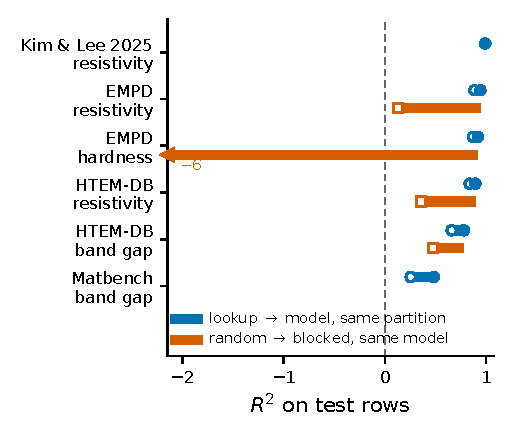
\includegraphics{figures/split_vs_model}
\caption{Under a random partition, the lookup reaches most of the model's $R^2$
on each property of each combinatorial dataset. The bars show the model's
margin relative to the lookup under a random partition (upper bar, open circle
at the lookup and filled circle at the model) and the drop in the model's $R^2$
when whole libraries or alloy systems are excluded from training (lower bar,
open square at the blocked score). The lower bar is absent for the control dataset and for
Kim and Lee's dataset. HTEM-DB resistivity is modeled as its base-10 logarithm. The dashed line marks zero, the score of a constant predictor returning the mean
target. The two circles of Kim and Lee's dataset overlap at
this scale. If the left edge of the axis cuts a bar short, the bar ends in
an arrow labeled with the bar's blocked score.}
\label{fig:split}
\end{figure}

\begin{table}[p]
\footnotesize
\setlength{\tabcolsep}{3pt}
\caption{The lookup and the model, per dataset and property. Each $R^2$ is a
mean over \splitDraws\ partitions, except that Kim and Lee's files define one
partition and we use one blocked partition of HTEM-DB. Bracketed ranges
are \bootstrapLevel\% percentile bootstrap intervals over
\bootstrapReplicates\ resamples, of libraries for the HTEM-DB rows, of compounds
for the Matbench row, and of the \splitDraws\ partitions for the EMPD rows.}
\label{tab:main}
% Generated from the committed result files; not hand-edited.
\textbf{(a) Under a random partition of the rows.}\\[3pt]
\begin{tabular*}{\textwidth}{@{\extracolsep{\fill}}lrlrrl}
\hline
dataset and property & rows & group & lookup $R^2$ & model $R^2$ & model $-$ lookup \\
\hline
Kim \& Lee 2025, resistivity & \npjDatasetRows & \npjSystems\ systems, not recorded & \npjLookupRSq & \npjModelRSq & \npjMargin \\
EMPD, resistivity & \empdResRows & \empdResSystems\ systems & \empdResLookup & \empdResModel & \empdResMargin~\empdResMarginCI \\
EMPD, hardness & \empdHardRows & \empdHardSystems\ systems & \empdHardLookup & \empdHardModel & \empdHardMargin~\empdHardMarginCI \\
HTEM-DB, resistivity & \htemResRows & \htemResLibraries\ libraries & \htemResRandomLookup & \htemResRandomModel & \htemResMargin~\htemResMarginCI \\
HTEM-DB, band gap & \htemGapRows & \htemGapLibraries\ libraries & \htemGapRandomLookup & \htemGapRandomModel & \htemGapMargin~\htemGapMarginCI \\
Matbench, band gap & \exptGapRows & no libraries & \exptGapLookup & \exptGapModel & \exptGapMargin~\exptGapMarginCI \\
\hline
\end{tabular*}

\vspace{10pt}

\textbf{(b) Under a blocked partition.}\\[3pt]
\begin{tabular*}{\textwidth}{@{\extracolsep{\fill}}lrll}
\hline
dataset and property & lookup $R^2$ & model $R^2$ & excess \\
\hline
EMPD, resistivity & \empdResBlockedLookup~\empdResBlockedLookupCI & \empdResBlocked~\empdResBlockedCI & \empdResExcess~\empdResExcessCI \\
EMPD, hardness & \empdHardBlockedLookup~\empdHardBlockedLookupCI & \empdHardBlocked~\empdHardBlockedCI & \empdHardExcess~\empdHardExcessCI \\
HTEM-DB, resistivity & \htemResBlockedLookup~\htemResBlockedLookupCI & \htemResBlockedModel~\htemResBlockedModelCI & \htemResExcess~\htemResExcessCI \\
HTEM-DB, band gap & \htemGapBlockedLookup~\htemGapBlockedLookupCI & \htemGapBlockedModel~\htemGapBlockedModelCI & \htemGapExcess~\htemGapExcessCI \\
\hline
\end{tabular*}

\end{table}

\end{document}
